  {\large \fontB Description:}
  
  {\bf solCA} is a 2-dimensional analytical solution to the Cauchy equations with the acceleration term set to zero
  to represent creeping flow. The boundary conditions are free-slip everywhere on a unit domain. The viscosity is constant.
  The flow is driven by a dense column centred at $ x=x_0 $ of width $dx$.
  \\

 {\large \fontB Parameters:}
  
 The variable parameters of this solution are:
 \begin{itemize}
   \item{density parameter: $ \sigma $.}
   \item{constant viscosity: $\eta$.}
   \item{width of dense column: $dx$.}
   \item{centre of dense column: $x_0$.}

 \end{itemize}

  \begin{SCfigure}[][h]
    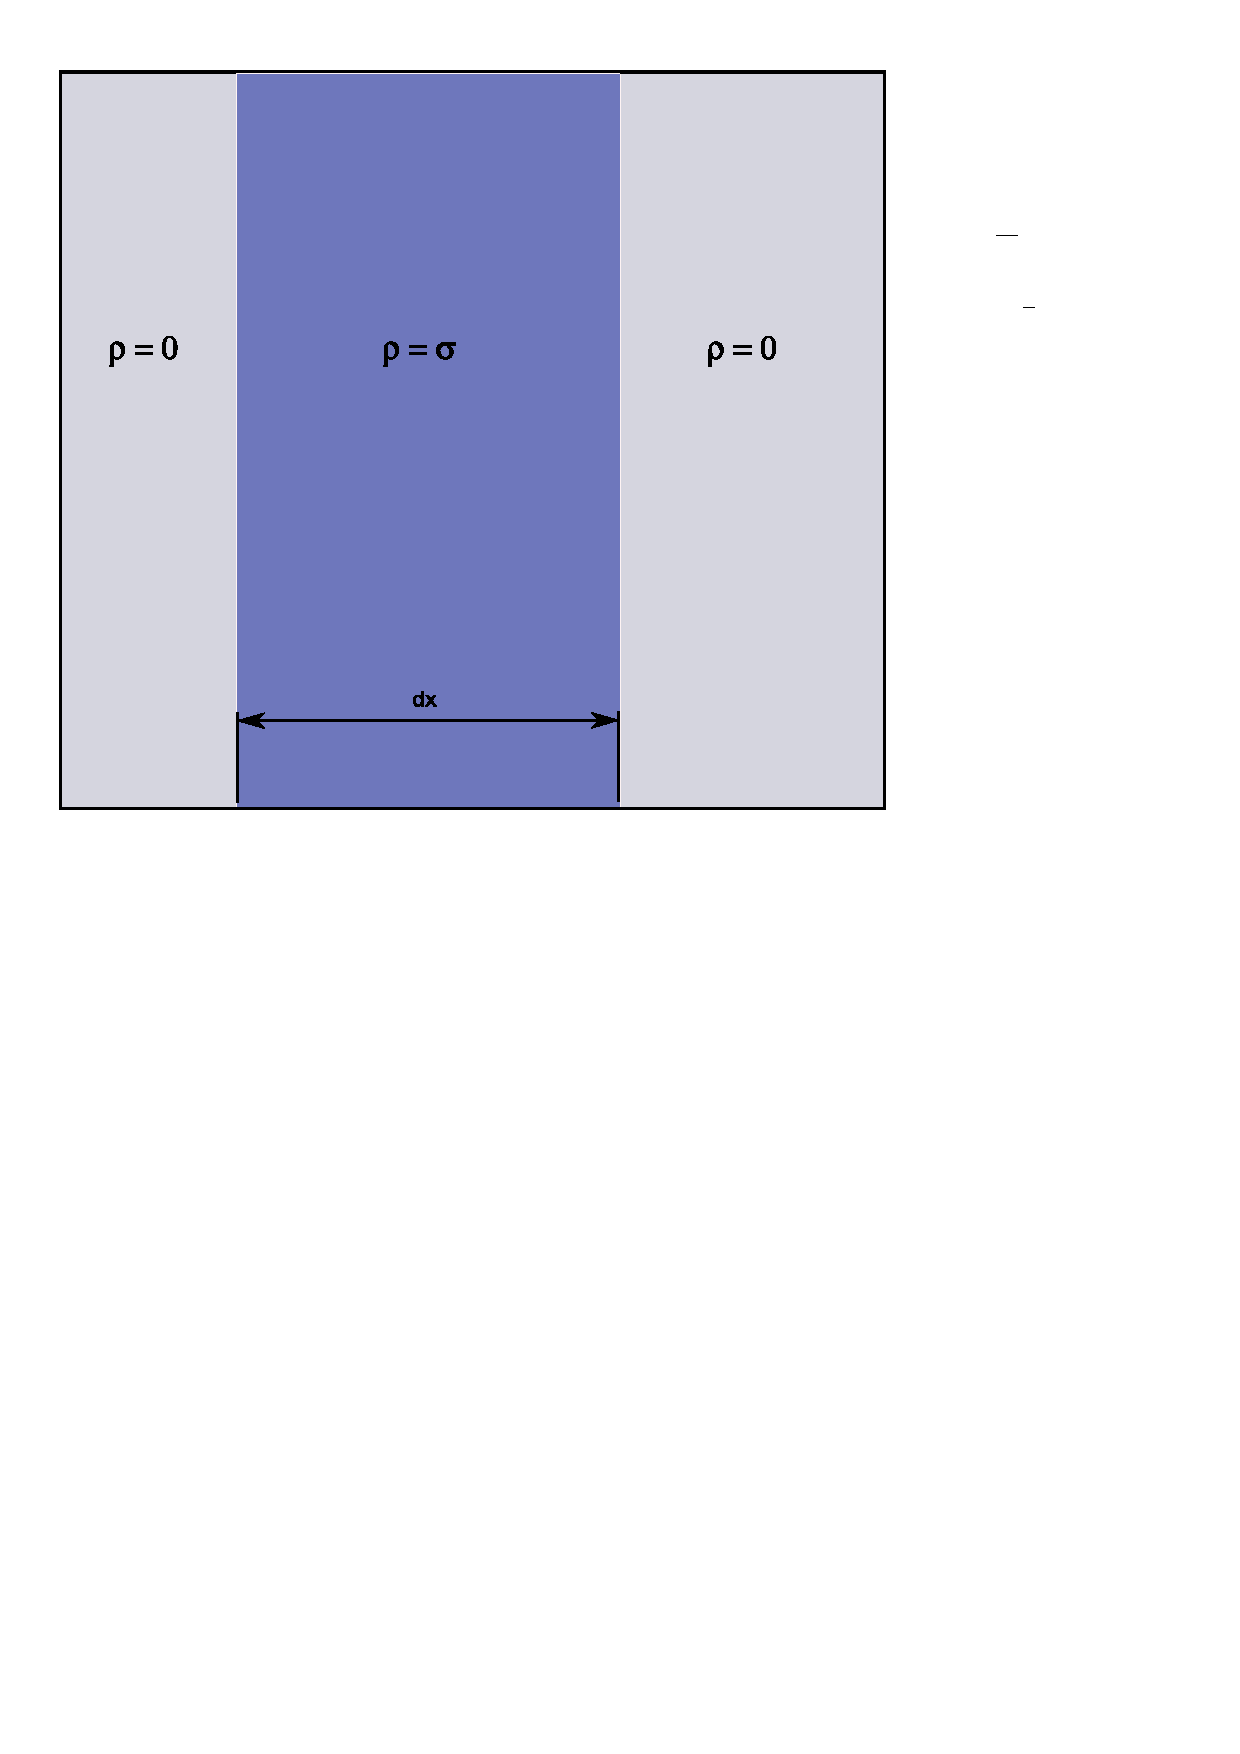
\includegraphics[width=6cm,clip]{../figs/figCA}
    \caption[Short caption]{\label{figCA} 
      Solution ({\bf SolCA}):
      This solution has a column of density $\rho = \sigma$ from $x_0-dx/2 < x < x_0+dx/2$.
      It is isoviscous.
      The boundary conditions are free slip everywhere on the surfaces of the unit box.}
  \end{SCfigure} 
  

